\documentclass{article}

\usepackage{graphicx}
\usepackage{caption}
\usepackage{subcaption}
\usepackage{hyperref}
\usepackage{listings}

\begin{document}

\title{
    Assignment 1 - Copy models for data compression \\
    \large{Algorithmic Information Theory (2022/23) \\
    Universidade de Aveiro}
}

\author{
    Martinho Tavares, 98262, martinho.tavares@ua.pt \and
    Nuno Cunha, 98124, nunocunha@ua.pt \and
    Pedro Lima, 97860, p.lima@ua.pt
}

\date{\today}
\maketitle

\section{Introduction}

One of the goals of this assignment is to implement a copy model for data compression, which is obtained through the exploration of self similarities.
A copy model is only one of the ways to address the problem, and its idea is that certain data sources can be viewed as a sequence of repetitive patterns,
where parts of the data have been replicated in the past, although some modifications are possible. 
The model consists in predicting the next symbol based on previous ones observed in the past, by keeping a pointer referring to the symbol being copied, as well as other information.

The second goal of the assignment is to implement a text generator based on the copy model, which is a way to generate new text based on a given one.
The text generator receives a text as input to train the model, and then follows a similar approach to the one used in the copy model,
but instead of predicting the next symbol, it uses the probability distribution to generate a random symbol based on these probabilities.

In this report we will first present how the work was organized, in the \ref{sec:work-organization} section.
Then, we will present the \ref{sec:copy-model}, how we implemented it and the results obtained, which we will compare by calculating the entropy of different text examples,
like \verb|chry.txt| given by the teachers, with different parameters we defined for the model.
The next section is dedicated to the \ref{sec:text-generator}, where we will present the implementation and the results obtained for the text generator,
using different texts as input for training of the generator, as well as diferrent starting points for the generation of text.
Finally, we will conclude the report in the \ref{sec:conclusion} section.

\section{Work organization}
\label{sec:work-organization}

To organize the work we decide to use a object oriented approach, this way it was easier to implement different parameters to test the copy model and the text generator.

First for the copy model we created a file named \verb|main.cpp|, where we instantiate the object \verb|CopyModel|, which is the class that implements the copy model.
The \verb|CopyModel| class has a constructor that receives the parameters that we want to test, and with these parameters we can instantiate different objects of certain classes, and test them with different files.
The more important classes are the abstract classes: \verb|CopyPointerManager|, \verb|CopyPointerThreshold| and \verb|BaseDistribution|. By using these base classes we could implement different strategies for the copy model, by creating child classes of these base classes, and then instantiate the \verb|CopyModel| object with the child classes as parameters.
This proved to be a very useful approach, since we could test different strategies for the copy model, and compare the results obtained to see which strategy, or combination of strategy/parameters, was the best.

For the text generator all the code is in the \verb|cpm_gen.cpp| file, due to its more simple structure. The generator also implements some parameters and uses a similar strategy of reading patterns as the copy model.

\section{Copy model}
\label{sec:copy-model}

The copy model behaves in a straightforward way.
At each symbol in the file, the program verifies if the pattern of $k$ symbols with the current symbol being the last has already occurred in the past.
That is, at position $x_n$, the pattern within positions $x_{n-k+1}$ and $x_n$ is evaluated to see if it appeared in the past.

To do that, each of these $k$-sized patterns at every position is saved in a hash table built incrementally while the file is being processed.
The keys are the $k$mers/patterns, and the values are arrays of positions in the file where those $k$mers occurred in the past, which we call pointers.
When we need to choose a pattern in the past, we look through the array of pointers for that pattern for a specific occurrence of that pattern.

Whenever the pattern is still not present in the hash table, we try to randomly guess which symbol should occur next since we can't perform a copy from the past.
In these cases, the reported probabilities follow a fixed default distribution that is set beforehand.

When predictions can be made, a strategy is followed to choose the appropriate pointer for the current pattern.
After a pointer is chosen, it is fixed and predictions are made sequentially from that point on.
That is, if at position $x_n$ we have the copy pointer $x_m$, then we will predict the character at $x_{n+1}$ to be equal to the character at $x_{m+1}$, the character at $x_{n+2}$ to be equal to the character at $x_{m+2}$, and so on.
The predictions aren't completely certain; we assume a probability of making a correct prediction, which varies depending on how well the prediction going.

This process is repeated until a threshold is met, which is based on the probability of making a correct prediction at the current position.
When the threshold is met, we stop predicting, and keep evaluating the file's content as normal.
If the current $k$mer has already occurred in the past, then we attempt a new chain of predictions.
Otherwise, we perform guesses.

We need to be careful regarding the beginning of the file.
For the first $k-1$ symbols, it is not possible to generate a $k$mer, but we should still be able to perform predictions starting on these $k-1$ symbols.
We followed a simple strategy, which involves extending the file content backwards, generating a past of size $k$.
The generated past is simple, it is composed of $k$ repetitions of a single symbol of the alphabet.
This symbol is the most frequent of the entire alphabet.

In order to evaluate whether the copy model can provide acceptable results, we can use a baseline below which we expect the model to report the file's entropy.
We decided to use, as a baseline, the entropy considering each symbol's relative frequency in the entire file, which is given by:

$$
H(X) = - \sum_{x \in X}{p(x) \log{p(x)}}
$$

With this value in mind, we evaluated the model as a whole with different values for its parameters, on different files.
The files chosen for testing are present in the repository\footnote{\url{https://github.com/NMPC27/TAI-G7-Lab1}}, and they have the following baselines:
\begin{itemize}
    \item \verb|chry.txt|: \dots
    \item \verb|...|: \dots
\end{itemize}

Throughout this section, the different program parameters are detailed, and their effect on the model's performance, both in terms of execution time and quality of the results, is studied.

For the results regarding the information content of the symbols throughout the \verb|chry.txt| file, the data was transformed with a low-pass filter using a moving average, since there are too many data points.

\subsection{Pattern size}

When choosing a pointer in the past from which to start copying, we need to look for an occurrence of the same $k$-sized pattern as the one we are currently on.
Thus, $k$ is one of the parameters that affects program performance, where $k$ is a positive integer.

On one hand, a lower value of $k$ means there will be more occurrences of each pattern, since there will be lesser possible $k$-sized patterns, which will result in more oportunities to copy from the past.
On the other, a larger $k$ will cause less occurrences for each pattern, which results in more scarce predictions, and thus more overall guesses.

For a given $k$, the number of possible patterns $M$ is equal to the number of permutations of the symbols of alphabet $A$: $M = \vert A \vert ^ k$.
The results on changing this value will be studied taking this exponential growth into account.

\subsubsection{Results}

\dots

\subsection{Smoothing parameter alpha}

At each coding step, the probability of correctly predicting the current character is given by the formula:

$$
P(\textnormal{hit}) = \frac{N_h + \alpha}{N_h + N_f + 2\alpha}
$$

where $N_h$ and $N_f$ are respectively the number of hits and misses, and $\alpha$ is the smoothing parameter.
The smoothing parameter is used to avoid the model having a probability of 0 when there are no hits or misses, which will happen when no prediction has been made yet, and also avoid assuming with complete certainty (probability of 1) that the prediction will be correct when no fails were made yet, which will result in infinite information in case the prediction fails.

If $\alpha$ is lower, we expect the reported probabilites to be more ``certain'' with a greater possibility of reaching high values.
If $\alpha$ is greater, the smoothing effect should be more pronounced, producing probability values that hardly increase, which should result in relatively less information when predictions fail but also lesser returns on the correct predictions.

This trade-off between $\alpha$ and the reported information, especially regarding the information spikes that may occur, will be studied in the results.

\subsubsection{Results}

\dots

\subsection{Base probability distribution}

For each symbol in the file, a probability distribution has to be generated according to the prediction probability.
In case a given prediction fails, we need to distribute the complement of the probability of a correct prediction $1 - P(\textnormal{hit})$ among the other symbols of the alphabet, except the one that we predicted would occur (which has probability $P(\textnormal{hit})$).

The choice of distribution also influences the guesses that are made.
When a prediction can't be made, the model assumes a distribution for the entirety of the alphabet, which is the same probability distribution as the use used when distributing the complement of the prediction probability.

We developed two simple approaches to distributing the probability: a uniform distribution and a frequency distribution.

The uniform distribution assigns to each symbol a probability equal to:

$$
\frac{1 - P(\textnormal{hit})}{\vert A \vert - 1}
$$

On the other hand, the frequency distribution assigns to each symbol $a \in A$ a probability equal to:

$$
(1 - P(\textnormal{hit})) \times p(a)
$$

where $p(a)$ is the probability of $a$ in the whole file.

Both distributions are compared especially in their effect on the overall reported information, when $k$ is large and thus more guesses are made, as well as when $\alpha$ is large and the prediction fails should report.
We assume that, since the frequency distribution models the overall distribution of the symbols, it should provide better results.
We should note, however, that the file's content may have locality, i.e. select portions in the file where the symbol distribution is skewed.
Therefore, we don't disregard the possibility that the assumption of the distribution being maintained throughout the file can hurt the model performance as well.

\subsubsection{Results}

\dots

\subsection{Copy pointer repositioning strategy}

Different strategies can be followed when choosing a copy pointer from which to start copying.
We developed 3 approaches, 2 of which being fairly simplistic:
\begin{itemize}
    \item \textbf{Oldest pointer first}: the chosen copy pointer is the oldest possible. If the current copy pointer is repositioned because the threshold was met, then that pointer will be completely discarded and the next oldest pointer is used.
    This is the most simple approach, which assumes similar patterns are very far in the file;
    \item \textbf{Newest pointer first}: the chosen copy pointer is always the newest, which assumes that similar patterns are very close in the file;
    \item \textbf{Most common prediction}: when a pointer has to be chosen, the predictions of all registered pointers are evaluated, and the pointer (or one of them) which presented longest and most common prediction is chosen.
    A more detailed description of this strategy is presented below.
    \item \textbf{Most common prediction bounded}: the approach is exactly the same as the \textbf{most common prediction}, with the only difference being that the registered pointers for each pattern are stored in a circular array with limited size.
\end{itemize}

The \textbf{most common prediction} strategy chooses the copy pointer in successive iterations.
Initially, the next immediate character is evaluated for every registered pointer.
The pointers are grouped according to that character that they predict, and the largest group is chosen, i.e. the pointers that reported the most common prediction are chosen.
Afterwards, the second next character is evaluated for every pointer in that group, and then the pointers are grouped in the same manner again, with the next group being the largest at this stage.
This process is repeated until all pointers at the current group report different predictions, at which point the newest pointer is chosen.

In order to obtain the most common prediction at each iteration, the Boyer-Moore majority vote algorithm was used \cite{majority}.
This is a very space-efficient algorithm (complexity $O(1)$) that guarantees the majority value will be returned.
However, if a majority value doesn't actually exist then the algorithm may erroneously report a value as the majority, if we only do one pass.
Since in this case we don't have a specific disambiguation strategy when the pointers don't agree, the choice is arbitrary and thus this is not a problem.

The bounded version of \textbf{most common prediction} uses a circular array for the set of registered pointers.
The idea is for the array of registered pointers to contain only the $N$ most recent pointers, with $N$ being the array size.
This can not only take into account the locality that the file's content may have, i.e. the repeated patterns being close to each other, but it also bounds the array size to a fixed value, which helps in performance since the reposition algorithm previously described has linear time complexity $O(N)$, when the other strategies have only $O(1)$ complexity.

\subsubsection{Results}

\begin{figure}

    \begin{subfigure}[b]{0.3\textwidth}
        \begin{center}
            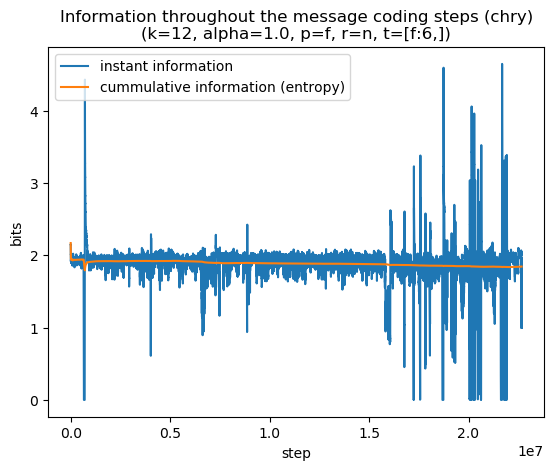
\includegraphics[width=1.0\linewidth]{../scripts/images/chry_12_1.0_f_n_[f:6,].png}
        \end{center}
        \caption{Oldest pointer first.}
        \label{fig:results-reposition-n}
    \end{subfigure}
    \hfill
    \begin{subfigure}[b]{0.3\textwidth}
        \begin{center}
            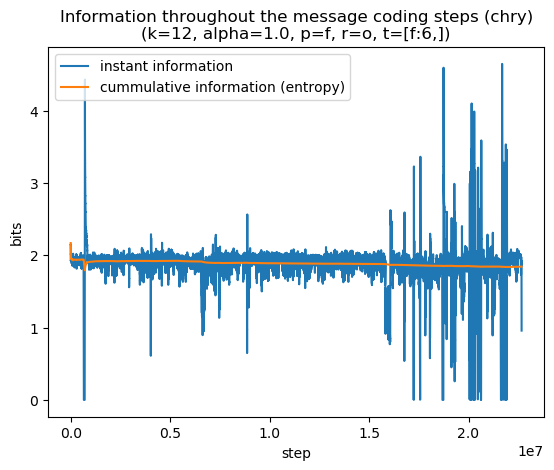
\includegraphics[width=1.0\linewidth]{../scripts/images/chry_12_1.0_f_o_[f:6,].png}
        \end{center}
        \caption{Newest pointer first.}
        \label{fig:results-reposition-o}
    \end{subfigure}
    \hfill
    \begin{subfigure}[b]{0.3\textwidth}
        \begin{center}
            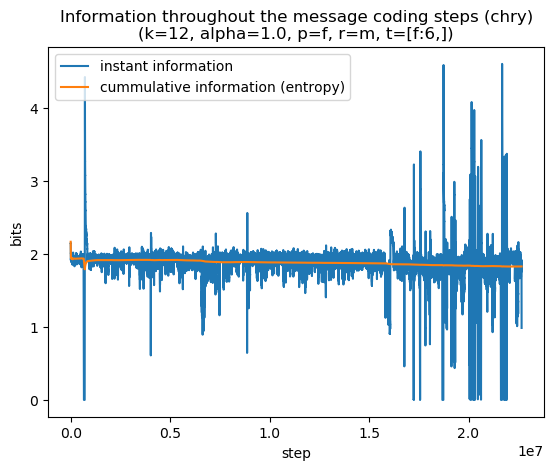
\includegraphics[width=1.0\linewidth]{../scripts/images/chry_12_1.0_f_m_[f:6,].png}
        \end{center}
        \caption{Most common prediction.}
        \label{fig:results-reposition-m}
    \end{subfigure}
    \caption{Information of the current symbol and entropy as the file is processed, varying the pointer reposition strategy.}
    \label{fig:results-reposition}
\end{figure}

\subsection{Copy pointer reposition threshold}

A copy pointer is used until the predictions are deemed to not be worthwhile.
After that point, the copy pointer is repositioned taking the current pattern into account.
The decision of when to reposition the copy pointer can be done using different approaches.

We developed 3 strategies, all of which only factor in the prediction probability over time:
\begin{itemize}
    \item \textbf{Static}: a static probability threshold value. If the prediction probability falls below this value, then the pointer is repositioned.
    \item \textbf{Successive fails}: if the number of successive prediction misses is larger than a given value, then the pointer is repositioned.
    In this case, the ``successive fails'' are evaluated using a non-negative counter of misses that is updated as predictions are made; whenever there is a miss, the counter increases, and decreases otherwise.
    \item \textbf{Rate of change}: if the absolute difference between the current prediction probability and the previous prediction probability is below a threshold then the pointer is repositioned.
\end{itemize}

Each strategy has a threshold value associated with them, and they are passed as parameters along with the specified strategy.
These thresholds can also be combined together, indicating whether the pointer should be repositioned when at least one of the strategies reports that their threshold was surpassed.

\subsubsection{Results}

The results were initially evaluated for each strategy in isolation.
After determining the best performing threshold values for each approach, they were combined among themselves, testing the 4 possible combinations.

\dots

\subsection{Verbose output}

As a sidenote, the model offers the possibility of outputting the probability distributions and predicitons at each step, or of presenting the overall progress of processing the input file.

For the modes outputting the probabilities, the output can be in human-readable format, presenting whether the reported probabilites were from a guess or a prediction hit/miss in colored output.
Alternatively, the output can be presented as comma-separated values with less extraneous characters in machine-readable format, which is useful for data analysis afterwards.


\section{Text generator}
\label{sec:text-generator}

The Generator module makes use of the functionalities offered by the CPM module.
This module uses a Context Model calculated from a received text to calculate the
next characters based on a context phrase. 

It contains two main methods, the \verb|firstPass()|, that reads the training file and makes an initial pass through the text to calculate the frequencies of the characters.
This method also makes an context model based on the training file, and the size of the context is defined by the input string. 

The \verb|cpm_gen()| method uses the context model in the first pass to generate the text.
When we try to generate the next symbol, we read the current context, which is the size of the input string and we check the context model for that context. If we have that context in the model, we get the list of possible next symbols, and their counts. Then, we generate a random value between 0 and the sum of the counts, and we check where that value lands between all the ranges of counts of events of that context. The symbol that is in the range of the random value is the next symbol of the text.
If we don't have that context in the model, we get the list of all possible symbols in the alphabet, and their distribution, and we generate a random value between 0 and the sum of the distributions, and we check where that value lands between all the ranges of distributions of events of that context. The symbol that is in the range of the random value is the next symbol of the text. 

We also have 2 other input parameters that modify the behavior of the generator. The first one is allowing the model to train itself, while generating the text. This is done by updating the context model with the generated text and the distibution of symbols in the alphabet.
The second parameter is to allow all lowercase characters to be generated, this is done by converting all the characters to lowercase while reading the training file. This parameter provides a better context model without needing a big training file, but it also makes the text generated to be all lowercase.


\subsection{Results}


Results for the text generator without -l or -t parameters:

\hfill

Listing 1: Generator output for train file "othello.txt" with initial string "T" and without -l or -t parameters
\\Num guesses: 0

\begin{lstlisting}
----------------------------------------------------------
Houllo m  oue he plled th So taby t want,   ke tirrad:
----------------------------------------------------------
\end{lstlisting}

Listing 2: Generator output for train file "othello.txt" with initial string "Th" and without -l or -t parameters
\\Num guesses: 0

\begin{lstlisting}
----------------------------------------------------------
I the my And him, Iager'd and th
----------------------------------------------------------
\end{lstlisting}

Listing 3: Generator output for train file "othello.txt" with initial string "The" and without -l or -t parameters
\\Num guesses: 0

\begin{lstlisting}
----------------------------------------------------------
Canitiall with Office. But that Cassio's see spokes.
----------------------------------------------------------
\end{lstlisting}

Listing 4: Generator output for train file "othello.txt" with initial string "The " and without -l or -t parameters
\\Num guesses: 0

\begin{lstlisting}
----------------------------------------------------------
Othello's Let to obey too much a round it, I thinke.
----------------------------------------------------------
\end{lstlisting}

Listing 5: Generator output for train file "othello.txt" with initial string "The t" and without -l or -t parameters
\\Num guesses: 0

\begin{lstlisting}
----------------------------------------------------------
I would them. And yet went busie must be Iago. Liue Rodo. 
With this?
----------------------------------------------------------
\end{lstlisting}

Listing 6: Generator output for train file "othello.txt" with initial string "The te" and without -l or -t parameters
\\Num guesses: 165

\begin{lstlisting}
----------------------------------------------------------
And marke how he comes to make a word or two before 
apprehend her faire Island,

Dc dHmr i aeihe, ooeelde smgimfpwi ? 
----------------------------------------------------------
\end{lstlisting}

Listing 7: Generator output for train file "othello.txt" with initial string "The tes" and without -l or -t parameters
\\Num guesses: 8 311

\begin{lstlisting}
----------------------------------------------------------
Do'st thou hast no name the Instruments summon to supper 
time

hatw,es  eegpa  rdlia vlnanrias in o ry ESowmn b syess g 
lant nero ue 
----------------------------------------------------------
\end{lstlisting}

Listing 8: Generator output for train file "othello.txt" with initial string "The test" and without -l or -t parameters
\\Num guesses: 10 000

\begin{lstlisting}
----------------------------------------------------------
one en,eLmosiuhnunrgtlveecm.n .aulebalom hdrd
----------------------------------------------------------
\end{lstlisting}



Results for the text generator with -l parameter:


\hfill

Listing 1: Generator output for train file "othello.txt" with initial string "T" and with -l parameter
\\Num guesses: 0

\begin{lstlisting}
----------------------------------------------------------
e, t t fllfod is pe ale mout thort g ld da meli s area 
vperd
----------------------------------------------------------
\end{lstlisting}

Listing 2: Generator output for train file "othello.txt" with initial string "Th" and with -l parameter
\\Num guesses: 0

\begin{lstlisting}
----------------------------------------------------------
dosto th torieuers: and fat cryther so yet so:
----------------------------------------------------------
\end{lstlisting}

Listing 3: Generator output for train file "othello.txt" with initial string "The" and with -l parameter
\\Num guesses: 0

\begin{lstlisting}
----------------------------------------------------------
and timentena some rod. if that now he drunke more ete. 
lord?
----------------------------------------------------------
\end{lstlisting}

Listing 4: Generator output for train file "othello.txt" with initial string "The " and with -l parameter
\\Num guesses: 0

\begin{lstlisting}
----------------------------------------------------------
my wife: i would nothinkings. what i will men othello, 
take thy awl'd thing.
----------------------------------------------------------
\end{lstlisting}

Listing 5: Generator output for train file "othello.txt" with initial string "The t" and with -l parameter
\\Num guesses: 0

\begin{lstlisting}
----------------------------------------------------------
rodo. patience. let's go safely by breake no iago. 'faith 
one cases,
----------------------------------------------------------
\end{lstlisting}

Listing 6: Generator output for train file "othello.txt" with initial string "The te" and with -l parameter
\\Num guesses: 0

\begin{lstlisting}
----------------------------------------------------------
why stand i loue be now to dyet my lippes: is't you cassio 
be receiu'd her father,
----------------------------------------------------------
\end{lstlisting}

Listing 7: Generator output for train file "othello.txt" with initial string "The tes" and with -l parameter
\\Num guesses: 7 899

\begin{lstlisting}
----------------------------------------------------------
that i can discourse. which they iumpe not one, that 
sweete othello?

wuo og,ahwolseh.eu afet hfmgath saegnnr hisdsdhaaiin
----------------------------------------------------------
\end{lstlisting}

Listing 8: Generator output for train file "othello.txt" with initial string "The test" and with -l parameter
\\Num guesses: 9 229

\begin{lstlisting}
----------------------------------------------------------
mus. i marry. what? a custome: but in a man that latest, 
which not enriches him,

tt oitdi ?w,ehyas a lw n rhge hayo
----------------------------------------------------------
\end{lstlisting}



Results for the text generator with -t parameter:


\hfill

Listing 1: Generator output for train file "othello.txt" with initial string "T" and with -t parameter
\\Num guesses: 0

\begin{lstlisting}
----------------------------------------------------------
So Ieread atle m bo. wathin o. Lino Whe Ansois. tes sh.
----------------------------------------------------------
\end{lstlisting}

Listing 2: Generator output for train file "othello.txt" with initial string "Th" and with -t parameter
\\Num guesses: 0

\begin{lstlisting}
----------------------------------------------------------
We sioneues, makendinget want hon and, youry her.
----------------------------------------------------------
\end{lstlisting}

Listing 3: Generator output for train file "othello.txt" with initial string "The" and with -t parameter
\\Num guesses: 0

\begin{lstlisting}
----------------------------------------------------------
Iago. Why Minuation, that pray you know is Tempt is liues 
of it same
----------------------------------------------------------
\end{lstlisting}

Listing 4: Generator output for train file "othello.txt" with initial string "The " and with -t parameter
\\Num guesses: 0

\begin{lstlisting}
----------------------------------------------------------
Exit Cas. I will you go with loue alread Rod. What breaken 
of Maine:
----------------------------------------------------------
\end{lstlisting}

Listing 5: Generator output for train file "othello.txt" with initial string "The t" and with -t parameter
\\Num guesses: 0

\begin{lstlisting}
----------------------------------------------------------
Othello: heereafter more next night, or his faire him at 
your Daughter
----------------------------------------------------------
\end{lstlisting}

Listing 6: Generator output for train file "othello.txt" with initial string "The te" and with -t parameter
\\Num guesses: 34

\begin{lstlisting}
----------------------------------------------------------
Des. It is now a huge Eclipse

a d sia r io a proper man: Oh, my face 
----------------------------------------------------------
\end{lstlisting}

Listing 7: Generator output for train file "othello.txt" with initial string "The tes" and with -t parameter
\\Num guesses: 6 533

\begin{lstlisting}
----------------------------------------------------------
How he vpbraides Iago, Attendants, with leade direction.

mpo gu hsees w?u a sfeesrso  hsnesatlAghhoif
----------------------------------------------------------
\end{lstlisting}

Listing 8: Generator output for train file "othello.txt" with initial string "The test" and with -t parameter
\\Num guesses: 10 000

\begin{lstlisting}
----------------------------------------------------------
s:cieBgt kofhb  afgeerarHlyuhm.rlwuy.ett u tihlA mmr'
inaaDnr nuI'oWanulo
----------------------------------------------------------
\end{lstlisting}

    
    

\section{Conclusion}
\label{sec:conclusion}


\section{References}
\bibliography{refs}
\bibliographystyle{IEEEtran}

\end{document}


